\documentclass[aspectratio=169]{beamer}

\usetheme{Madrid}
\usecolortheme{default}
\setbeamertemplate{navigation symbols}{}

\usepackage[T1]{fontenc}
\usepackage[utf8]{inputenc}
\usepackage{lmodern}
\usepackage{amsmath}
\usepackage{booktabs}
\usepackage{array}
\usepackage{tikz}
\usepackage{pgfplots}
\usepackage{graphicx}

\pgfplotsset{compat=1.18}

\definecolor{ODUNavy}{RGB}{17,47,78}
\definecolor{ODUTeal}{RGB}{48,116,122}
\definecolor{ODUSky}{RGB}{93,162,190}
\definecolor{ODULight}{RGB}{241,245,249}
\definecolor{ODUOrange}{RGB}{210,135,55}
\definecolor{ODUGreen}{RGB}{55,149,88}
\definecolor{ODURed}{RGB}{171,59,59}
\definecolor{ODUGray}{RGB}{84,92,101}

\setbeamercolor{structure}{fg=ODUNavy}
\setbeamercolor{frametitle}{fg=white,bg=ODUNavy}
\setbeamercolor{title}{fg=white,bg=ODUNavy}
\setbeamercolor{block title}{fg=white,bg=ODUNavy}
\setbeamercolor{block body}{fg=black,bg=ODULight}
\setbeamercolor{item projected}{fg=white,bg=ODUTeal}

\setbeamertemplate{title page}{
  \vfill
  \begin{center}
    \begin{beamercolorbox}[wd=\textwidth,ht=3.0cm,dp=0pt,center]{title}
      \vbox to 3.0cm{
        \vfil
        \usebeamerfont{title}\inserttitle\par
        \vfil
      }
    \end{beamercolorbox}

    \vspace{1.1em}
    {\usebeamerfont{author}\insertauthor\par}
    \vspace{0.35em}
    {\usebeamerfont{institute}\insertinstitute\par}
    \vspace{0.35em}
    {\usebeamerfont{date}\insertdate\par}
  \end{center}
  \vfill
}

\title{Signalized Intersection Simulator Project}
\author{Dr. Kun Xie}
\institute{Old Dominion University}
\date{\today}

\newcommand{\metricbox}[3]{
  \begin{tikzpicture}
    \node[
      draw=#1,
      rounded corners=4pt,
      line width=0.9pt,
      fill=white,
      minimum width=3.3cm,
      minimum height=1.55cm,
      align=center
    ] {
      {\scriptsize #2} \\
      \vspace{0.12cm}
      {\large\bfseries #3}
    };
  \end{tikzpicture}
}

\begin{document}

\begin{frame}
  \titlepage
\end{frame}

\begin{frame}{Presentation Outline}
  \tableofcontents
\end{frame}

\section{Problem}
\begin{frame}{Problem and Motivation}
  \begin{columns}[T,totalwidth=\textwidth]
    \column{0.58\textwidth}
    \begin{block}{Why this project matters}
      \begin{itemize}
        \item Traffic signal timing, queueing, and delay are often introduced analytically before students can see the dynamics directly.
        \item A browser-based simulator provides an accessible way to connect theory with observable operational behavior.
        \item The project focuses on conceptual understanding and classroom experimentation rather than field calibration.
      \end{itemize}
    \end{block}

    \column{0.38\textwidth}
    \begin{beamercolorbox}[rounded=true,shadow=false,sep=1em,wd=\textwidth]{block body}
      \textbf{Guiding question}

      \vspace{0.4em}
      How do signal timing, stochastic arrivals, turning movements, and vehicle mix influence queue growth and delay at a four-leg intersection?
    \end{beamercolorbox}
  \end{columns}
\end{frame}

\section{Methodology}
\begin{frame}{Methodology}
  \begin{enumerate}
    \item Define user inputs: east-west green, yellow, north-south green, arrival rates by approach, free-flow speed, left-turn ratio, large-vehicle ratio, and simulation speed.
    \item Generate arrivals stochastically for each approach to represent demand variability.
    \item Update a two-phase signal controller that alternates east-west and north-south service.
    \item Move vehicles using lane-based trajectories, car-following logic, and permissive left-turn yielding against opposing through traffic.
    \item Report performance in real time using arrivals, departures, current queue, average queue, maximum queue, and average delay.
  \end{enumerate}

  \vspace{0.5em}
  \begin{beamercolorbox}[rounded=true,sep=0.7em,wd=\textwidth]{block body}
    \textbf{Modeling emphasis:} The simulator is intentionally lightweight, but it still captures the interaction between control, demand, and vehicle behavior clearly enough for teaching purposes.
  \end{beamercolorbox}
\end{frame}

\section{Design}
\begin{frame}[shrink=4]{Simulation Design}
  \begin{columns}[T,totalwidth=\textwidth]
    \column{0.48\textwidth}
    \textbf{Intersection geometry and control}
    \begin{itemize}
      \item Four-leg signalized intersection
      \item One inbound lane on each approach
      \item Two-phase signal with adjustable yellow clearance
      \item Left, through, and right turning movements
    \end{itemize}

    \begin{center}
    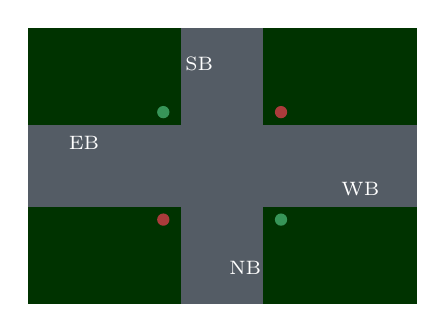
\begin{tikzpicture}[scale=0.65]
      \fill[green!20!black] (-3.8,-2.7) rectangle (3.8,2.7);
      \fill[ODUGray] (-3.8,-0.8) rectangle (3.8,0.8);
      \fill[ODUGray] (-0.8,-2.7) rectangle (0.8,2.7);

      \fill[ODUGreen] (-1.15,1.05) circle (0.12);
      \fill[ODURed] (1.15,1.05) circle (0.12);
      \fill[ODURed] (-1.15,-1.05) circle (0.12);
      \fill[ODUGreen] (1.15,-1.05) circle (0.12);

      \node[white] at (-2.7,0.45) {\scriptsize EB};
      \node[white] at (2.7,-0.45) {\scriptsize WB};
      \node[white] at (-0.45,2.0) {\scriptsize SB};
      \node[white] at (0.45,-2.0) {\scriptsize NB};
    \end{tikzpicture}
    \end{center}

    \column{0.48\textwidth}
    \textbf{Software and metrics}
    \begin{itemize}
      \item HTML/CSS/JavaScript front end
      \item Animated canvas-based visualization
      \item Queue detection from stopped or trapped vehicles
      \item Delay based on completed trips relative to free-flow travel time
    \end{itemize}

    \vspace{0.5em}
    \begin{block}{User-facing outputs}
      Arrivals, departures, queue, average queue, maximum queue, average delay, signal state, and simulation clock.
    \end{block}
  \end{columns}
\end{frame}

\section{Results}
\begin{frame}[shrink=6]{Illustrative Results}
  \centering
  \metricbox{ODUOrange}{Baseline average delay}{50.6 s/veh}
  \hspace{0.2cm}
  \metricbox{ODUTeal}{Baseline average queue}{14.7 veh}
  \hspace{0.2cm}
  \metricbox{ODUSky}{Baseline maximum queue}{31.5 veh}
  \hspace{0.2cm}
  \metricbox{ODUNavy}{Baseline throughput}{1569.6 veh/h}

  \vspace{0.5cm}

  \begin{columns}[T,totalwidth=\textwidth]
    \column{0.54\textwidth}
    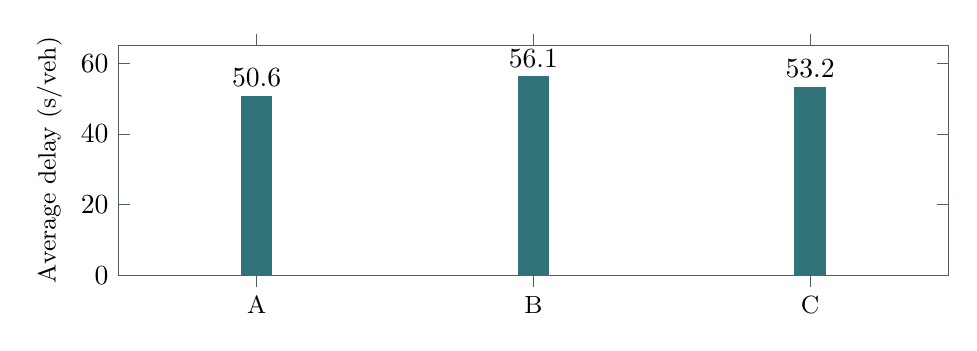
\begin{tikzpicture}
      \begin{axis}[
        width=\linewidth,
        height=4.5cm,
        ybar,
        bar width=11pt,
        ymin=0,
        ymax=65,
        ylabel={Average delay (s/veh)},
        symbolic x coords={A,B,C},
        xtick=data,
        nodes near coords,
        nodes near coords align={vertical},
        enlarge x limits=0.25,
        axis line style={draw=ODUGray},
        tick style={draw=ODUGray},
        ylabel style={font=\small},
        xticklabel style={font=\small}
      ]
        \addplot[fill=ODUTeal,draw=ODUTeal] coordinates {(A,50.6) (B,56.1) (C,53.2)};
      \end{axis}
    \end{tikzpicture}

    \column{0.42\textwidth}
    \small
    \textbf{Scenario definitions}
    \begin{itemize}
      \item A: Balanced demand, timing 30-5-30
      \item B: Heavy east-west demand, timing 30-5-30
      \item C: Heavy east-west demand, retimed to 40-5-20
    \end{itemize}

    \vspace{0.4em}
    \textbf{Experimental setup}
    \begin{itemize}
      \item 10 replications per scenario
      \item 1,200 simulated seconds per run
      \item Results are illustrative outputs from the teaching simulator
    \end{itemize}
  \end{columns}
\end{frame}

\begin{frame}{Scenario Comparison}
  \small
  \begin{table}
    \centering
    \begin{tabular}{>{\raggedright\arraybackslash}p{2.3cm} >{\centering\arraybackslash}p{2.2cm} >{\centering\arraybackslash}p{2.4cm} >{\centering\arraybackslash}p{2.2cm} >{\centering\arraybackslash}p{2.3cm}}
      \toprule
      Scenario & Timing & Avg. Delay & Avg. Queue & Throughput \\
      \midrule
      A: Balanced demand & 30-5-30 & 50.6 s/veh & 14.7 veh & 1569.6 veh/h \\
      B: Heavy EW demand & 30-5-30 & 56.1 s/veh & 16.5 veh & 1515.0 veh/h \\
      C: Heavy EW retimed & 40-5-20 & 53.2 s/veh & 15.7 veh & 1615.5 veh/h \\
      \bottomrule
    \end{tabular}
  \end{table}

  \vspace{0.5em}
  \begin{block}{Interpretation}
    Increasing east-west demand without retiming raises delay and queueing. Reallocating green time to the dominant approaches improves performance, which shows that the simulator can support comparative signal timing analysis in addition to visualization.
  \end{block}
\end{frame}

\section{Future Work}
\begin{frame}{Future Work}
  \begin{columns}[T,totalwidth=\textwidth]
    \column{0.32\textwidth}
    \begin{block}{Model Enhancements}
      \begin{itemize}
        \item Protected left-turn phasing
        \item Additional lane groups
        \item Pedestrian calls and more detailed clearance logic
      \end{itemize}
    \end{block}

    \column{0.32\textwidth}
    \begin{block}{Validation and Analysis}
      \begin{itemize}
        \item Calibration against field observations
        \item Batch experiments with confidence intervals
        \item Comparison with deterministic HCM-style calculations
      \end{itemize}
    \end{block}

    \column{0.32\textwidth}
    \begin{block}{Instructional Features}
      \begin{itemize}
        \item Saved classroom scenarios
        \item Guided student experiments
        \item Phase timelines and queue heatmaps
      \end{itemize}
    \end{block}
  \end{columns}
\end{frame}

\begin{frame}{Conclusion}
  \begin{itemize}
    \item The traffic simulator provides a compact and accessible teaching tool for signalized intersection operations.
    \item Its structure is simple enough for classroom use, but still rich enough to demonstrate timing, demand imbalance, queueing, and delay.
    \item The Beamer deck presents the project in an academic format suitable for class, lab, or project presentation.
  \end{itemize}

  \vfill
  \centering
  {\Large Thank you}
\end{frame}

\end{document}
